\section{Theoretische Grundlage}
\label{sec:Theorie}
\subsection{Ziel}
Ziel des Versuches ist es der elastisches Modul eines Metalls mittels einer Drehschwingung zu bestimmten, als auch das magnetische Moment eines Permanentmagneten.
\subsection{Normal-, Schubspannung und Hooksches Gesetz}
Kräfte die an die Oberfläche eines elastischen Körper angreifen, verformen diesen. Aufgrund dessen werden die Größe Spannung definiert, welche ein Verhältniss von der Kraft zum ein Flächenelement herstellt.
\begin{equation}
  \sigma = \frac{F}{m^2} \, \frac{\text{N}}{m^2}
  \label{eqn:Spannung}
\end{equation}
Sie lassen sich in zwei Kategorien aufteilen. Als Normalspannung $\sigma_\text{N}$ werden die Kräfte bezeichnet welche senkrecht zur Oberfläche stehen. Die Kräfte welche parallel zur Oberfläche stehen heißen Schubspannung $\sigma_\text{S}$. Desweiteren gibt es noch Volumenkräfte. Bei solchen greift die Kraft an jedem Volumenelement an, zum Beispiel die Schwerkraft.

Zwischen hinreichend kleinen Spannungen und Deformation besteht ein proportionaler Zusammenhang welcher als Hooksches bezeichnet wird.
\begin{equation}
  \sigma = E \frac{\Delta L}{L}  \hspace{2em} \text{und} \hspace{2em} P = Q\frac{\Delta V}{V}
  \label{eqn:Hook}
\end{equation}
Um alle Spannungen in einem Kristall volständig zu beschreiben werden jeweils 6 Komponenten benötigt, wobei 3 für die Gestaltsund 3 für die Volumenelastizität zuständig sind. Bei einem einfachen  Kristall mit niedriger Symmetrie entsteht deswegen eine 6x6-Matrix mit 36 Einträgen. Bei kubischen Kristallen lässt sich aufgrund der symmetrie der Matrix und des Körpers auf 3 Einträge verringern. Handelt sich zusätzlich um einen isotropen Körper, so lässt sich der Körper vollständig durch 2 Konstanten beschreiben.

\subsection{Elastische Konstanten isotroper Stoffe}
Zur Berechnung des elastizitschen Konstanten wird einerseits die Torsionsmodul $G$ als auch das Komprssionsmodul $Q$ benötigt bzw das Elastizitätsmodul $\sigma$.
Die Poissonsche Querkontraktionszahl µ Verknüpft die Längenänderung mit der Normalspannung. Die Abbildung \ref{fig:poisson} soll die anhand eines einseitig eingespannten Stab verdeulichen.
\begin{figure}
  \centering
  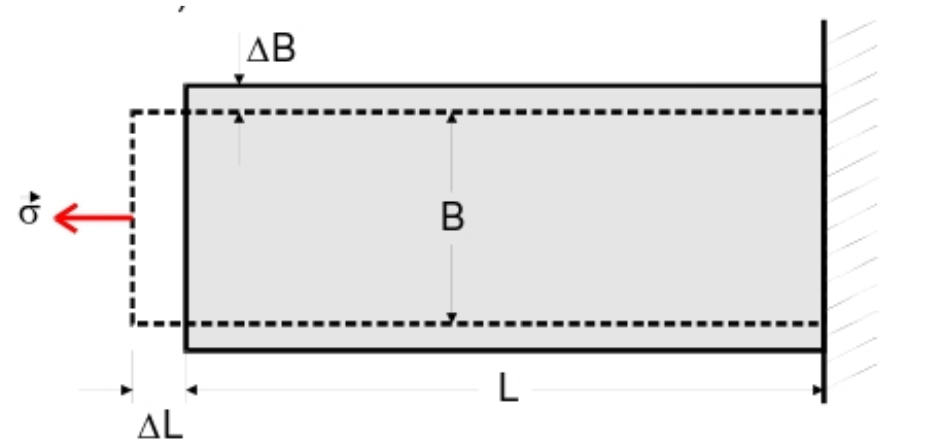
\includegraphics[width=5.0cm]{./picture/poisson.png}
  \caption{<+caption text+>}
  \label{fig:poisson}
\end{figure}
\begin{equation}
  \text{µ} := -\frac{\Delta B}{B} \cdot \frac{L}{\Delta L} = \frac{E}{2G} - 1
  \label{eqn:pois}
\end{equation}
Das Kompressionsmodul $Q$ berechnet sich aus dem Elastizitätsmodul so wie der Querkontraktionszahl µ.
\begin{equation}
  Q = \frac{E}{-6 \mu + 3}
  \label{eqn:komp}
\end{equation}

\subsection{Bestimmung des Torsionsmoduls G}
Um die elastische Nachwirkung vernachlässigen zu können, wird zur Bestimmung des Torsionsmoduls eine dynamische Methode gewählt. Als elastische Nachwirkung wird die Zeit benötigt bis gewisse Materialien nach einer Belastung wieder in ihren Ausgangszustandung zurückkehrt.
Für die Dynamische Methode wird ein zylinderförmiger Draht an einem Ende Eingespannt und auf der anderen Seite wirkt über ein Kräftepaar ein Drehmoment auf diesen. Durch die Scherung des Drahtes um den Winkel \alpha kommt es zu einer Drehmoment welche infitesimalen Drehmomente über den Radius des Zylinders  integriert werden.
\begin{equation}
  M = \frac{\pi G R^4 \varphi}{2L} =: D \varphi
  \label{eqn:M}
\end{equation}
In Analogie zur Federkonstante wird $D$ als Richtgröße bezeichnet. Durch eine kleine Auslenkung aus der Ruhelage im Rahmen der Kleinwinkelnäherung lässt sich das Schwingungsfähige System durch die Differentialgleichung
\begin{equation}
  D \varphi + \theta \varphi = 0
  \label{eqn:dgl}
\end{equation}
beschreiben, wobei \theta das Trägheitsmoment des Systems ist. Der Differnentialgleichung wird eine Periodendauer von
\begin{equation}
  T = 2 \pi \sqrt{\frac{\theta}{D}}
  \label{eqn:T}
\end{equation}
entnommen und das Trägheitsmoment der Kugel aud des Formel
\begin{equation}
  \theta_\text{Kugel} = \frac{2}{5}m_\text{k}R_\text{k}^2
  \label{eqn:theta}
\end{equation}
berechnet. Somit ergibt sich aus Formel \ref{eqn:M}, \ref{eqn:T} und \ref{eqn:theta} ein Torsionsmodul $G$ von
\begin{equation}
  G = \frac{16 \pi m_\text{k} R_\text{k}^2 L}{5 T^2 R^4} \ .
  \label{eqn:G}
\end{equation}
\subsection{Magnetisches Moment eines Permanentmagnetens}
Das magnetische Moment $\vec{m}$  eine Permanentmagneten ist definiert als
\begin{equation}
  \vec{m} := p \vec{a}
  \label{eqn:m}
\end{equation}
wobei $p$ die Polstärke und $\vec{a}$ die Abstände der beiden Pole ist. Auf dem Magneten wirkt in einem B-Feld wie in Abbildung ?? zu sehen, dass Magnetische Moment $M_\text{Mag}$ zweier entgegengesetzter Kräfte. Der Betrag des magnetische Momentens ist
\begin{equation}
  |M_\text{Mag}| = m B sin(\gamma)
  \label{eqn:MM}
\end{equation}
Daraus ergibt sich die nicht lineare Differentialgleichung
\begin{equation}
  mBsin \varphi + D \varphi + \theta \frac{d^2 \varphi}{dt^2}
  \label{eqn:idgl}
\end{equation} welche sich jedoch durch die Kleinwinkelnäherung $sin \varphi \sim \varphi$ in eine homogene Umschreiben lässt. Daraus lässt sich die Schwingungsdauer
\begin{equation}
  T_\text{Mag} = 2 \pi \sqrt{\frac{\theta}{mB + D}}
  \label{eqn:Tmag}
\end{equation}
entnehmen.
\subsection{Fehlerrechnung}
\subsubsection{Mittelwert}
Der Mittelwert einer Messreihe $x_\text{1}, ... ,x_\text{n}$ lässt sich durch die Formel
\begin{equation}
	\overline{x} = \frac{1}{N} \sum_{\text{k}=1}^\text{N} x_k
	\label{eqn:ave}
\end{equation}
berechnen. Die Standardabweichung des Mittelwertes beträgt
\begin{equation}
	\Delta \overline{x} = \sqrt{ \frac{1}{N(N-1)} \sum_{\text{k}=1}^\text{N} (x_\text{k} - \overline{x})^2}
	\label{eqn:std}
\end{equation}

\subsubsection{Fehlerfortpflanzung}
Die Fehlerfortpflanzung übernimmt Python 3.4.3 mit der Funktion "ufloat" aus "Python-Uncertainties".

\subsubsection{Lineare Regression}
Die Lineare Regression und sämtliche andere Rechnungen wurden ebenfalls mit Python 3.4.3 durchgeführt.
